\documentclass[12pt]{article}
\usepackage{graphicx}
\usepackage{enumerate}
\usepackage{booktabs}
\usepackage[T1]{fontenc}
\author{Aaron Song s267807}
\title{CW2}
\date{\today}


\begin{document}
\maketitle



\section{Task 1}

1. An entry of data in this problem is defined as $(x,y,label)$, where $x$ and $y$ is the inputs and $label$ is the output. Define:
\begin{description}
    \item[data] Data: x:number, y:number, label: number
    \item[neural network] A neural network in this task is an object with a function that takes a pair of numbers of outputs a number, so functionally define Apply: number->number->number and NeuralNetwork: { Apply }.
    \item[loss function] Loss(nn: NeuralNetwork, d: Data) = $((\textrm{Apply d.x d.y)-d.error)}^2$
    \item[fitness functtion] The fitness of a neural network is the average loss on the specific dataset. $$Ftiness(nn: NeuralNetwork, ds: Data[]) = \frac{\sum_{i=1}^{\textrm{ds.Length}}Loss(nn, ds[i])}{ds.Length}$$
\end{description}

\noindent 2. A [-10, 10] is enough for this question.

\noindent 3. Two hidden layers are used, with the first 5~7 neurons and the second 2 neurons. If only one hidden layer is permitted, 7 neurons are prefered to get a better result, as shown in Figure \ref{7n}.\\
With PSO, as shown in Figure \ref{pso_7n}, the best result achieved is the test loss of 0.119. The performance is much worser than stochastic gradient descent.
\begin{figure}[!ht]
\centering
\begin{minipage}[t]{0.48\textwidth}
    \centering
    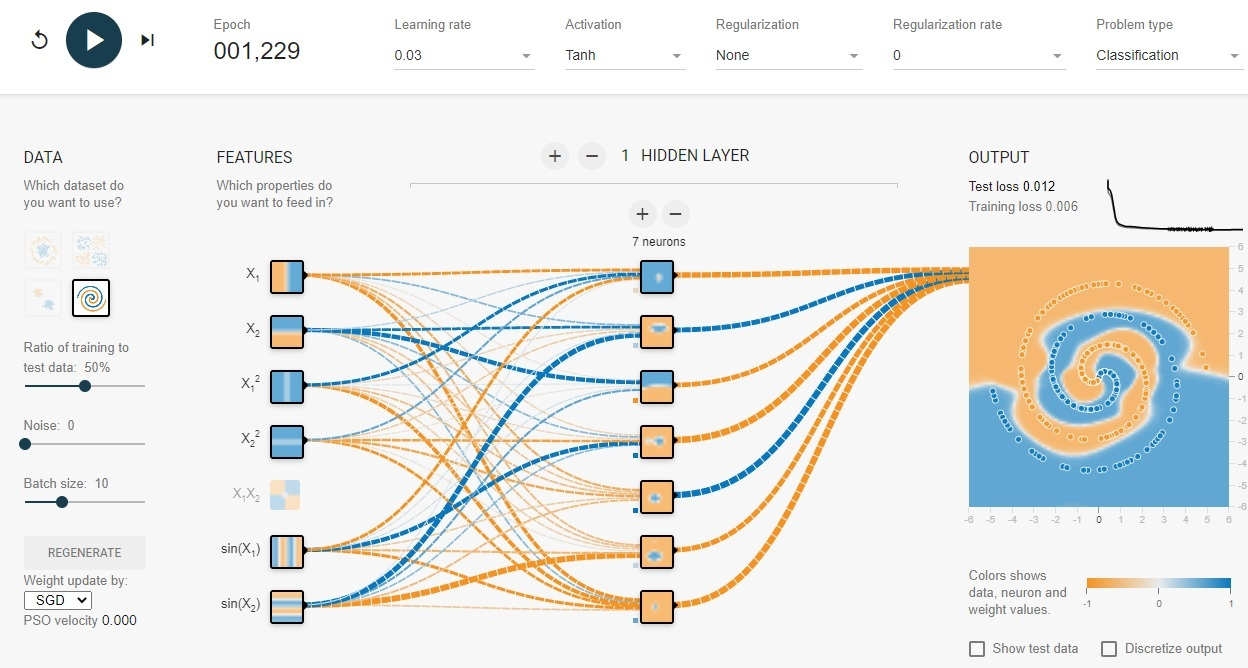
\includegraphics[width=\textwidth]{1.jpg}
    \caption{A hidden layer with 7 neurons}
    \label{7n}
\end{minipage}
\begin{minipage}[t]{0.48\textwidth}
    \centering
    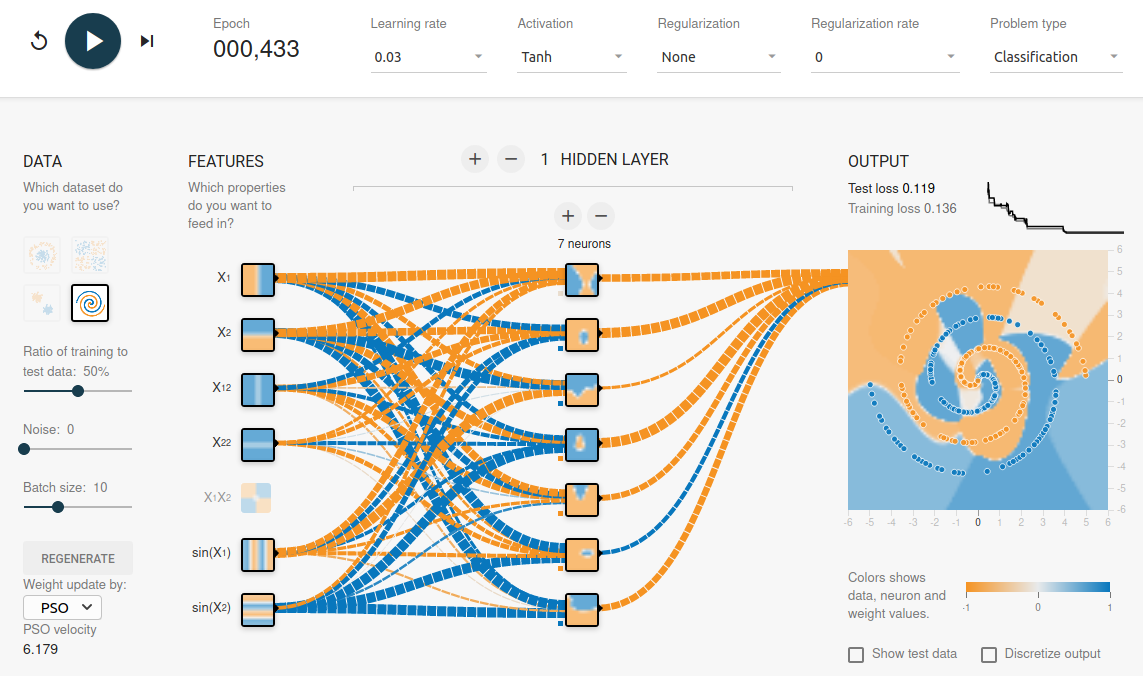
\includegraphics[width=\textwidth]{PSO.png}
    \caption{Using PSO to optimize weights}
    \label{pso_7n}
\end{minipage}
\end{figure}


\noindent 4.
The learning result is much better when non-linear input are involved. For this question specifically, a spiral data is generated by a formula $r=k\theta$ where $k>0, \theta>0$. When translating the polar coordinate into a Cartisean coordinate, it's 
\begin{equation}
\label{equ:task1-target-func}
\sqrt{x^2+y^2}=k(2n\pi+\textrm{atan2}(x,y))
\end{equation}
, where $n\in Z$ and atan2 is the arctan function defined by most common programming language where the range is $[0,2\pi)$. In order to expand the aforementioned equation into a plain form, atan2 can be approximately translated into $\arctan$, and according to Tylor expansion, 
\begin{equation}
    \frac{\textrm{d}\arctan x}{\textrm{d}x}=\frac{1}{x+1}\\
\arctan x=x-\frac{1}{3}x^3+\frac{1}{5}x^5-\ldots
\end{equation}
. Curtailling high order terms, 
$$
\arctan x=x-\frac{1}{3}x^3\\
x^2+y^2=an+b(x-\frac{1}{3}x^3)^2
$$
where $a=\frac{4k^2}{\pi^2},b=k^2$. Curtailling high order terms again, 
$$
x^2+y^2=an+bx
$$
We can see that $x^2$, $y^2$, terms are presented here. To fully simulate the spiral data generation function \ref{equ:task1-target-func}, $\sin x$ and $\sin y$ may also be included given the Tylor expansion:
$$
\sin x=x-\frac{1}{3!}x^3+\frac{1}{5!}x^5-\ldots
$$

\noindent 5. Many NN parameters have an effect to this particular problem.
\begin{description}
    \item[learning rate] The learning rate decides how fast the weights and biases of the neural network changes. A moderate value (0.03 or 0.1) yields good output, otherwise if it's too high ($\geq 1$) the training loss and the test lost will fluctuate too fast and fail to converge to a proper local best. If too small ($\leq 0.0003$), the weights and the biases barely change. A global best may still present itself after enough long time, but that may take too many epochs.
    \item[activation function] Activation function is used to discretse the floating-number output of the neural network into a number. The default activation tanh in this problem suits very well, and sigmoid also fits good despite longer training time may be required. RBF and ReLU are also acceptable. Sin doesn't fit well since the radius is not constant, and linear doesn't work at all.
    \item[regularisation]
    \item[feature] The features in this problem are the soul source of non-linear input and decide the form of the neural network; the number of layers and the number of neurons on each layer depend only the linear combination of the input features. As memtioned in the previous question, $x_1^2$ and $\sin x$ improve the learning result a lot compared to a purely linear model. I also tried $x_1^3$ and $x_2^3$, but the result is not satisfying.
    \item[nn shape] Every neural node blends all inputs linearly and yields one single value. Mathematically, suppose there are $x$ layers (including the input layer) of nodes in the neural network and on layer $i$ there are $k[i]$ nodes ($0\leq i<x$), then node $b$ on layer $0<a\leq x$ $n_{a,b}$ takes a vector 
    $X=(x_0,x_1,\ldots,x_{k[a-1]})$ as input and output $A\cdot X+B$, where $A$ stands for the weight between $a-1$ layer and node $n_{a,b}$ and $B$ represents the bias of node $n_{a,b}$.\\
    In other words, the input layer is defined by some common function $y=x$, $y=x^2$, $y=\sin x$, and nodes in a following layers form a linear combination of the last layer.
    
      
\end{description}
\noindent 6. The effect of the PSO parameters.
\begin{description}
\item[Inertia weight $\omega$]  $\omega$ is the weight that is given to the previous velocity. Tuning $\omega$ will affect the balance between exploitation and exploration. If $\omega = 0$, particles will only move toward personal best and global best. If $\omega > 0$, the particles will have some exploitation of local space. \\
There is an experiment of different $\omega$ choice on a NN with 1 hidden layer, input features [$x_1,x_2,x_1^2,x_2^2,\sin(x_1),\sin(x_2)$], learning rate = 0.03, activation = Tanh, no regularization. $\alpha_1=\alpha_2 = 1.5$, swarm size = 100.
Results shown in Table \ref{t_omega}.
\begin{table}[h]
\centering
\begin{tabular}{@{}cccc@{}}
\toprule
$\omega$ & Average Test Loss & Epoches before stable \\ \midrule
0 & 0.43 & 50  \\
0.5 & 0.33  &  100  \\
0.7 & 0.22  &   400 \\
1  & 0.48  & Not Stable  \\
\bottomrule
\end{tabular}
\caption{Performance with different $\omega$}
\label{t_omega}
\end{table}
\\
The higher $\omega$, the more epoches are required to converge. If $\omega = 1$, the particles will keep on flying with increasing volocity.\\
Due to the stochastic of PSO, the test loss is not same at each run. 
\end{description}
\begin{description}
\item[accelerate constant $\alpha_1$ and $\alpha_2$ ] 

$\alpha_1$ and $\alpha_2$ describe the acceleration toward personal best and global best of a particle.
Small acceleration may cause the particles to fly around the goal area, and large acceleration may result in particle moving fast to the goal or even pass away from goal. If $\alpha_1 = 0$, the particle has no self-awareness, and will always get to new search space. It may converge faster, but it could lead to local minima. If $\alpha_2=0$, there is no interaction among particles, the particles will move alone. It probably won't converge.
Typically, $\alpha_1 = \alpha_2$.

\begin{table}[h]
\centering
\begin{tabular}{@{}cccc@{}}
\toprule
$\alpha_1$,$\alpha_2$ & Average Test Loss & PSO velocity \\ \midrule
1 & 0.36 & 3 to 5  \\
1.5 & 0.22  &  6 to 10  \\
2 & 0.39  &   7 to 12 \\
5  & 0.48  &  40 to 50  \\
\bottomrule
\end{tabular}
\caption{Performance with different $\alpha$}
\label{t_alpha}
\end{table}
The higher $\alpha$, the higher velocity of PSO.
If $\alpha_1 = 0$, the velocity reaches to 0 rapidly, but the test loss is above 0.5. If $\alpha_2 = 0$, the velocity does not reach to 0, but it is also worse than a random algorithm.

\end{description}
\begin{description}
\item[swarm size]
Swarm size is the number of particles. Larger swarm size could improve accuracy in difficult problems. Swarm size can critically affect the iteration time of an epoch.
\begin{table}[h]
\centering
\begin{tabular}{@{}cccc@{}}
\toprule
Swarm Size & Average Test Loss  \\ \midrule
10 & 0.32 \\
30 & 0.32    \\
100 & 0.22  \\
1000  & 0.22   \\
\bottomrule
\end{tabular}
\caption{Performance with different swarm size}
\label{t_swarm}
\end{table}
\end{description}

\begin{description}
\item[minimum and maximum velocity]
This is not implemented in the Playground, but it might have some influence. If the velocity is large, the particle may skip an optimum solution. If it is too small, the particle may get stuck with local minima.
\end{description}

\section{Task 2}
1. There're seven input nodes so the encoding of the input layer would be a binary string with a length of 7; the maximum number of layers is 6 and on each layer the limit of the number of neurons is 8, so a layer can be encoded in a binary string with a length of 3. In the first layer (also the input layer), every node is different because each one represents a different input function (it is however possible to have to input nodes with the same function, but it would be meaningless); for other layers, every node (neuron) is the same. So the neural network can be represented as:
$$
{i_0i_1\ldots i_7,\ l_{1_0}l_{1_1}l_{1_2},\ l_{5_0}l_{5_1}l_{5_2},\ \ldots,\ l_{6_0}l_{6_1}l_{6_2}}
$$
. 


\end{document}